\documentclass[a4paper,10pt]{article}

\usepackage{appendixnumberbeamer}
\usepackage{booktabs}
\usepackage[scale=2]{ccicons}
\usepackage{pgfplots}
\usepackage{xspace}
\usepackage{bookmark}
\usepackage{amssymb}
\usepackage{mathtools}
\usepackage[normalem]{ulem}
\usepackage[T1]{fontenc}
\usepackage[sfdefault,book]{FiraSans}
\usepackage{FiraMono}
\usepackage{fontawesome}
\usepackage{listings}
\usepackage{hyperref}
\usepackage[10pt]{moresize}

\renewcommand*\familydefault{\ttdefault}

\renewcommand{\thefootnote}{\fnsymbol{footnote}}
\renewcommand{\MintedPygmentize}{/home/thiago/.local/bin/pygmentize}

\definecolor{light-gray}{gray}{0.95}
\renewcommand\lstlistingname{Código}
\DeclareCaptionFormat{listing} {
  \parbox{\textwidth}{\hspace{-0.2cm}#1#2#3}
}
\DeclareCaptionFont{black}{\color{black}}
\captionsetup[lstlisting]{
  format=listing,
  labelfont=black,
  textfont=black,
  singlelinecheck=true,
  margin=0pt,
  font={tt,footnotesize,bf}
}

\lstset{
  basicstyle=\footnotesize\ttfamily,
  escapeinside={\%*}{*)},
  mathescape=true,
  showspaces=false,
  showtabs=false,
  showstringspaces=false,%
  % backgroundcolor=\color{light-gray},
  rulesepcolor=\color{black},
  frame=shadowbox,
  literate=
  {á}{{\'a}}1 {é}{{\'e}}1 {í}{{\'i}}1 {ó}{{\'o}}1 {ú}{{\'u}}1
  {Á}{{\'A}}1 {É}{{\'E}}1 {Í}{{\'I}}1 {Ó}{{\'O}}1 {Ú}{{\'U}}1
  {à}{{\`a}}1 {è}{{\`e}}1 {ì}{{\`i}}1 {ò}{{\`o}}1 {ù}{{\`u}}1
  {À}{{\`A}}1 {È}{{\'E}}1 {Ì}{{\`I}}1 {Ò}{{\`O}}1 {Ù}{{\`U}}1
  {ä}{{\"a}}1 {ë}{{\"e}}1 {ï}{{\"i}}1 {ö}{{\"o}}1 {ü}{{\"u}}1
  {Ä}{{\"A}}1 {Ë}{{\"E}}1 {Ï}{{\"I}}1 {Ö}{{\"O}}1 {Ü}{{\"U}}1
  {â}{{\^a}}1 {ê}{{\^e}}1 {î}{{\^i}}1 {ô}{{\^o}}1 {û}{{\^u}}1
  {Â}{{\^A}}1 {Ê}{{\^E}}1 {Î}{{\^I}}1 {Ô}{{\^O}}1 {Û}{{\^U}}1
  {Ã}{{\~A}}1 {ã}{{\~a}}1 {Õ}{{\~O}}1 {õ}{{\~o}}1
  {œ}{{\oe}}1 {Œ}{{\OE}}1 {æ}{{\ae}}1 {Æ}{{\AE}}1 {ß}{{\ss}}1
  {ű}{{\H{u}}}1 {Ű}{{\H{U}}}1 {ő}{{\H{o}}}1 {Ő}{{\H{O}}}1
  {ç}{{\c c}}1 {Ç}{{\c C}}1 {ø}{{\o}}1 {å}{{\r a}}1 {Å}{{\r A}}1
  {€}{{\euro}}1 {£}{{\pounds}}1 {«}{{\guillemotleft}}1
  {»}{{\guillemotright}}1 {ñ}{{\~n}}1 {Ñ}{{\~N}}1 {¿}{{?`}}1
}

\setminted{
  fontsize=\footnotesize,
  style=xcode,
  frame=single,
  framesep=3\fboxsep,
  labelposition=topline,
}


\title{Prova AB2}
\posttitle{\end{center}}

\begin{document}

\maketitle

\emergencystretch 3em

\begin{itemize}[itemsep=0em]
  \item Não use celular/computador e não converse com ninguém, a prova é individual.
  \item Sinta-se à vontade para tirar dúvidas (\textbf{razoáveis}) ou pedir esclarecimentos sobre as questões.
  \item Use \textbf{letra legível}! não posso dar nota para algo que não consigo ler.
  \item Lembre-se de \textbf{assinar seu nome nas suas folhas}. Se usar \textbf{mais de uma} folha, \textbf{enumere cada página}.
  \item \textbf{Seja organizado:} especifique número e letra da questão que você está respondendo e deixe um espaço entre as respostas, para não ficar tudo amontoado. Você pode pegar mais folhas, se precisar.
\end{itemize}


NOME: \rule{.85\textwidth}{0.1mm}

\begin{multicols*}{2}
\setlength{\leftmargini}{0pt}
\begin{enumerate}
  \item (2,5 pt) Um \textit{grafo coroa} de seis vértices é definido por $V = \{a_1, a_2, a_3, b_1, b_2, b_3\}$ e $E = \{(a_i, b_j)$, para $i \neq j\}$. Esse grafo é \textit{não direcionado}.

  \begin{enumerate}
    \item (0,6 pt) Faça uma representação visual do grafo.
    %     u1 -- v2
    %    /       \
    %  v3         u3
    %    \       /
    %     u2 -- v1
    \item (0,6 pt) Faça a matriz de adjacência do grafo.
    %    u1 u2 u3 v1 v2 v3
    % u1 0  0  0  0  1  1
    % u2 0  0  0  1  0  1
    % u3 0  0  0  1  1  0
    % v1 0  1  1  0  0  0
    % v2 1  0  1  0  0  0
    % v3 1  1  0  0  0  0
    \item (0,6 pt) Faça as listas de adjacência do grafo.
    % u1->|v2||->|v3||-> NULL
    % u2->|v1||->|v3||-> NULL
    % u3->|v1||->|v2||-> NULL
    % v1->|u2||->|u3||-> NULL
    % v2->|u1||->|u3||-> NULL
    % v3->|u1||->|u2||-> NULL
    % \item Esse grafo é simples? % Sim
    \item (0,7 pt) Esse grafo é cíclico? Se sim, especifique os vértices que fazem parte do ciclo. % Sim. Todos os vértices fazem parte do ciclo.
  \end{enumerate}

  \item (3,0 pt) A imagem a seguir representa um \textit{grafo de Herschel}, com 11 vértices e 18 arestas.

  \begin{center}
    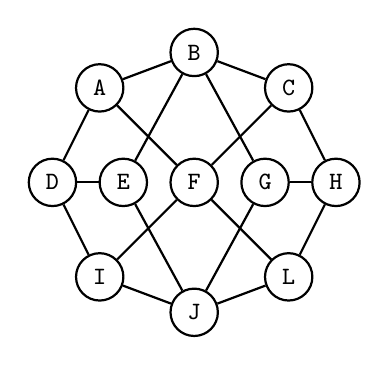
\begin{tikzpicture}[scale=0.6]
      \node[circle, draw=black, thick](A) at (-2.00, 2.00){\small A};
      \node[circle, draw=black, thick](B) at ( 0.00, 2.75){\small B};
      \node[circle, draw=black, thick](C) at ( 2.00, 2.00){\small C};
      \node[circle, draw=black, thick](D) at (-3.00, 0.00){\small D};
      \node[circle, draw=black, thick](E) at (-1.50, 0.00){\small E};
      \node[circle, draw=black, thick](F) at ( 0.00, 0.00){\small F};
      \node[circle, draw=black, thick](G) at ( 1.50, 0.00){\small G};
      \node[circle, draw=black, thick](H) at ( 3.00, 0.00){\small H};
      \node[circle, draw=black, thick](I) at (-2.00,-2.00){\small I};
      \node[circle, draw=black, thick](J) at ( 0.00,-2.75){\small J};
      \node[circle, draw=black, thick](L) at ( 2.00,-2.00){\small L};

      \draw[thick] (A) -- (B) -- (C) -- (H) -- (L) -- (J) -- (I) -- (D) -- (A);
      \draw[thick] (D) -- (E);
      \draw[thick] (G) -- (H);
      \draw[thick] (A) -- (F) -- (L);
      \draw[thick] (C) -- (F) -- (I);
      \draw[thick] (B) -- (E) -- (J) -- (G) -- (B);
    \end{tikzpicture}
  \end{center}

  \begin{enumerate}
    \item (1,2 pt) Faça uma BFS no grafo e obtenha a relação de parentesco entre os vértices, começando a partir do vértice E e explorando em ordem alfabética. Desenhe essa relação em um formato de árvore.
    %       ______(E)__
    %      /       |   \
    %   __(B)__   (D) (J)
    %  /   |   \   |   |
    % (A) (C) (G) (I) (L)
    %  |   |
    % (F) (H)
    %
    %  A  B  C  D  E  F  G  H  I  J  L
    %  B  E  B  E -1  A  B  C  D  E  J
    \item (0,8 pt) De acordo com o resultado da letra (a), qual é o caminho com menos arestas entre os vértices E e F? Cite outros dois caminhos entre os mesmos vértices e com a mesma quantidade de arestas que podem aparecer, caso a BFS seja feita com outras ordens de exploração.
    % E -> B -> A -> F
    % E -> B -> C -> F; E -> D -> A -> F
    \item (1,0 pt) Esse grafo é bipartido? Se sim, desenhe-o com os vértices coloridos. Caso contrário, mostre em que momento da BFS ocorre um conflito na hora de preencher as cores.
    % Sim.
    %    P--B--P
    %   / \/ \/ \
    %  /  /\ /\  \
    % B--P  B  P--B
    %  \  \/ \/  /
    %   \ /\ /\ /
    %    P--B--P
  \end{enumerate}

  \item (3,0 pt) As listas de adjacência a seguir representam um \textit{grafo de Moser}, com 7 vértices e 11 arestas. Esse grafo é \textit{não direcionado}.

  \begin{center}
    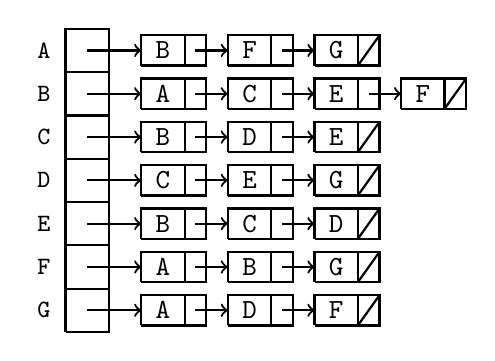
\begin{tikzpicture}[scale=0.55]
      \node[]() at (-1.00, 6.00){\small A};
      \node[]() at (-1.00, 5.00){\small B};
      \node[]() at (-1.00, 4.00){\small C};
      \node[]() at (-1.00, 3.00){\small D};
      \node[]() at (-1.00, 2.00){\small E};
      \node[]() at (-1.00, 1.00){\small F};
      \node[]() at (-1.00, 0.00){\small G};

      \node[](A) at ( 0.00, 6.00){};
      \node[](B) at ( 0.00, 5.00){};
      \node[](C) at ( 0.00, 4.00){};
      \node[](D) at ( 0.00, 3.00){};
      \node[](E) at ( 0.00, 2.00){};
      \node[](F) at ( 0.00, 1.00){};
      \node[](G) at ( 0.00, 0.00){};

      \draw[thick] (-0.50,-0.50) -- ( 0.50,-0.50) -- ( 0.50, 6.50) -- (-0.50, 6.50) -- (-0.50,-0.50);
      \draw[thick] (-0.50, 0.50) -- ( 0.50, 0.50);
      \draw[thick] (-0.50, 1.50) -- ( 0.50, 1.50);
      \draw[thick] (-0.50, 2.50) -- ( 0.50, 2.50);
      \draw[thick] (-0.50, 3.50) -- ( 0.50, 3.50);
      \draw[thick] (-0.50, 4.50) -- ( 0.50, 4.50);
      \draw[thick] (-0.50, 5.50) -- ( 0.50, 5.50);

      \draw[->, thick] (A.center) -- ++(1.25,0);
      \draw[->, thick] (B.center) -- ++(1.25,0);
      \draw[->, thick] (C.center) -- ++(1.25,0);
      \draw[->, thick] (D.center) -- ++(1.25,0);
      \draw[->, thick] (E.center) -- ++(1.25,0);
      \draw[->, thick] (F.center) -- ++(1.25,0);
      \draw[->, thick] (G.center) -- ++(1.25,0);

      \foreach \x\y in {0/A,1/A,2/B,3/C,4/B,5/A,6/B} {
        \draw[thick] (1.25,\x - 0.35) -- (1.25,\x + 0.35) -- (2.75,\x + 0.35) -- (2.75,\x - 0.35) -- (1.25,\x - 0.35) ;
        \draw[thick] (2.25,\x - 0.35) -- (2.25,\x + 0.35);
        \draw[->, thick] (2.50,\x) -- ++(0.75,0);
        \node[]() at (1.75, \x){\y};
      }

      \foreach \x\y in {0/D,1/B,2/C,3/E,4/D,5/C,6/F} {
        \draw[thick] (3.25,\x - 0.35) -- (3.25,\x + 0.35) -- (4.75,\x + 0.35) -- (4.75,\x - 0.35) -- (3.25,\x - 0.35) ;
        \draw[thick] (4.25,\x - 0.35) -- (4.25,\x + 0.35);
        \draw[->, thick] (4.50,\x) -- ++(0.75,0);
        \node[]() at (3.75, \x){\y};
      }

      \foreach \x\y in {0/F,1/G,2/D,3/G,4/E,5/E,6/G} {
        \draw[thick] (5.25,\x - 0.35) -- (5.25,\x + 0.35) -- (6.75,\x + 0.35) -- (6.75,\x - 0.35) -- (5.25,\x - 0.35) ;
        \draw[thick] (6.25,\x - 0.35) -- (6.25,\x + 0.35);
        \node[]() at (5.75, \x){\y};
      }

      \foreach \x\y in {0,1,2,3,4,6} {
        \draw[thick] (6.75,\x + 0.35) -- (6.25,\x - 0.35);
      }

      \draw[->, thick] (6.50, 5.00) -- ++(0.75,0);

      \draw[thick] (7.25,5.00 - 0.35) -- (7.25,5.00 + 0.35) -- (8.75,5.00 + 0.35) -- (8.75,5.00 - 0.35) -- (7.25,5.00 - 0.35) ;
      \draw[thick] (8.25,5.00 - 0.35) -- (8.25,5.00 + 0.35);
      \node[]() at (7.75, 5.00){F};
      \draw[thick] (8.75,5.00 + 0.35) -- (8.25,5.00 - 0.35);
    \end{tikzpicture}
  \end{center}

  \begin{enumerate}
    \item (1,2 pt) Faça uma DFS no grafo, começando a partir do vértice B e explorando em ordem alfabética \textit{inversa}. Obtenha a relação de parentesco entre os vértices e desenhe essa relação no formato de uma árvore.
    %    (B)
    %     |
    %    (F)
    %     |
    %    (G)
    %   /   \
    % (D)  (A)
    %  |
    % (E)
    %  |
    % (C)
    \item (0,8 pt) Classifique cada aresta do grafo.
    % A - B Retorno
    % A - F Retorno
    % A - G Árvore
    % B - C Retorno
    % B - E Retorno
    % B - F Árvore
    % C - E Árvore
    % C - D Retorno
    % D - E Árvore
    % D - G Árvore
    % F - G Árvore
    \item (1,0 pt) Transformando o grafo da questão em um DAG (\textit{grafo direcionado acíclico}), temos as listas de adjacência a seguir. Dê uma ordenação topológica para esse grafo.
    % G A F B E C D
  \end{enumerate}

  \begin{center}
    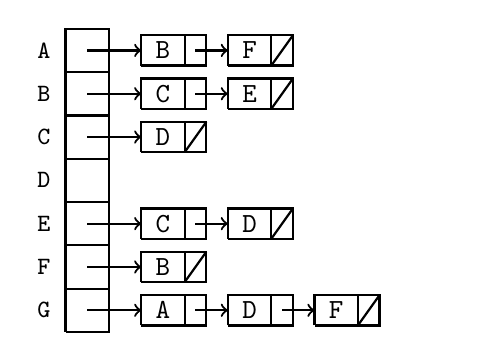
\begin{tikzpicture}[scale=0.55]
      \node[]() at (-1.00, 6.00){\small A};
      \node[]() at (-1.00, 5.00){\small B};
      \node[]() at (-1.00, 4.00){\small C};
      \node[]() at (-1.00, 3.00){\small D};
      \node[]() at (-1.00, 2.00){\small E};
      \node[]() at (-1.00, 1.00){\small F};
      \node[]() at (-1.00, 0.00){\small G};

      \node[](A) at ( 0.00, 6.00){};
      \node[](B) at ( 0.00, 5.00){};
      \node[](C) at ( 0.00, 4.00){};
      \node[](D) at ( 0.00, 3.00){};
      \node[](E) at ( 0.00, 2.00){};
      \node[](F) at ( 0.00, 1.00){};
      \node[](G) at ( 0.00, 0.00){};

      \draw[thick] (-0.50,-0.50) -- ( 0.50,-0.50) -- ( 0.50, 6.50) -- (-0.50, 6.50) -- (-0.50,-0.50);
      \draw[thick] (-0.50, 0.50) -- ( 0.50, 0.50);
      \draw[thick] (-0.50, 1.50) -- ( 0.50, 1.50);
      \draw[thick] (-0.50, 2.50) -- ( 0.50, 2.50);
      \draw[thick] (-0.50, 3.50) -- ( 0.50, 3.50);
      \draw[thick] (-0.50, 4.50) -- ( 0.50, 4.50);
      \draw[thick] (-0.50, 5.50) -- ( 0.50, 5.50);

      \draw[->, thick] (A.center) -- ++(1.25,0);
      \draw[->, thick] (B.center) -- ++(1.25,0);
      \draw[->, thick] (C.center) -- ++(1.25,0);
      % \draw[->, thick] (D.center) -- ++(1.25,0);
      \draw[->, thick] (E.center) -- ++(1.25,0);
      \draw[->, thick] (F.center) -- ++(1.25,0);
      \draw[->, thick] (G.center) -- ++(1.25,0);

      \foreach \x\y in {0/A,1/B,2/C,4/D,5/C,6/B} {
        \draw[thick] (1.25,\x - 0.35) -- (1.25,\x + 0.35) -- (2.75,\x + 0.35) -- (2.75,\x - 0.35) -- (1.25,\x - 0.35) ;
        \draw[thick] (2.25,\x - 0.35) -- (2.25,\x + 0.35);
        \node[]() at (1.75, \x){\y};
      }

      \foreach \x in {0,2,5,6} {
        \draw[->, thick] (2.50,\x) -- ++(0.75,0);
      }

      \foreach \x\y in {1,4} {
        \draw[thick] (2.75,\x + 0.35) -- (2.25,\x - 0.35);
      }

      \foreach \x\y in {0/D,2/D,5/E,6/F} {
        \draw[thick] (3.25,\x - 0.35) -- (3.25,\x + 0.35) -- (4.75,\x + 0.35) -- (4.75,\x - 0.35) -- (3.25,\x - 0.35) ;
        \draw[thick] (4.25,\x - 0.35) -- (4.25,\x + 0.35);
        \node[]() at (3.75, \x){\y};
      }

      \foreach \x in {0} {
        \draw[->, thick] (4.50,\x) -- ++(0.75,0);
      }

      \foreach \x\y in {2,5,6} {
        \draw[thick] (4.75,\x + 0.35) -- (4.25,\x - 0.35);
      }

      \foreach \x\y in {0/F} {
        \draw[thick] (5.25,\x - 0.35) -- (5.25,\x + 0.35) -- (6.75,\x + 0.35) -- (6.75,\x - 0.35) -- (5.25,\x - 0.35) ;
        \draw[thick] (6.25,\x - 0.35) -- (6.25,\x + 0.35);
        \node[]() at (5.75, \x){\y};
      }

      \foreach \x\y in {0} {
        \draw[thick] (6.75,\x + 0.35) -- (6.25,\x - 0.35);
      }

      \draw[white,thick] (8.75,5.00 + 0.35) -- (8.25,5.00 - 0.35);
    \end{tikzpicture}
  \end{center}

  \item (1,5 pt) Encontre a árvore geradora mínima do grafo a seguir usando o algoritmo de Kruskal. Escreva a ordenação das arestas usada no algoritmo. Ordene as arestas com mesmo peso usando a ordem alfabética.
  % B - C  8
  % C - H  8
  % D - I  8
  % A - B 10
  % B - C 10
  % C - D 10
  % D - E 10
  % F - G 10
  % G - H 10
  % H - I 10
  % I - J 10
  % B - H 13
  % C - I 13
  %
  % (A)----(B)----(C)----(D)----(E)
  %         |      |      |
  %         |      |      |
  % (F)----(G)    (H)    (I)----(J)

  \begin{center}
  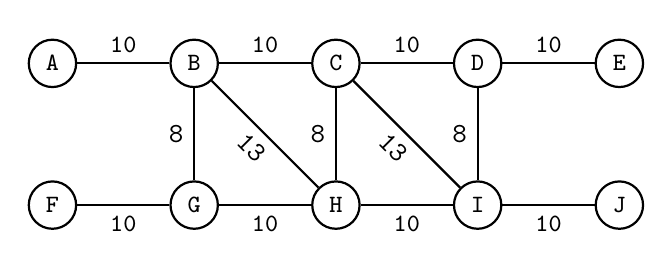
\begin{tikzpicture}[scale=0.9]
    \node[circle, draw=black, thick](A) at (0.00, 2.00){\small A};
    \node[circle, draw=black, thick](B) at (2.00, 2.00){\small B};
    \node[circle, draw=black, thick](C) at (4.00, 2.00){\small C};
    \node[circle, draw=black, thick](D) at (6.00, 2.00){\small D};
    \node[circle, draw=black, thick](E) at (8.00, 2.00){\small E};

    \node[circle, draw=black, thick](F) at (0.00, 0.00){\small F};
    \node[circle, draw=black, thick](G) at (2.00, 0.00){\small G};
    \node[circle, draw=black, thick](H) at (4.00, 0.00){\small H};
    \node[circle, draw=black, thick](I) at (6.00, 0.00){\small I};
    \node[circle, draw=black, thick](J) at (8.00, 0.00){\small J};

    \draw[thick] (A) -- node[anchor=south](){\small 10} (B) -- node[anchor=south](){\small 10} (C) -- node[anchor=south](){\small 10} (D) -- node[anchor=south](){\small 10} (E);
    \draw[thick] (F) -- node[anchor=north](){\small 10} (G) -- node[anchor=north](){\small 10} (H) -- node[anchor=north](){\small 10} (I) -- node[anchor=north](){\small 10} (J);

    \draw[thick] (B) -- node[anchor=east](){8} (G);
    \draw[thick] (C) -- node[anchor=east](){8} (H);
    \draw[thick] (D) -- node[anchor=east](){8} (I);

    \draw[thick] (B) -- node[anchor=north,rotate=-45](){13} (H);
    \draw[thick] (C) -- node[anchor=north,rotate=-45](){13} (I);
  \end{tikzpicture}
  \end{center}

\end{enumerate}
\end{multicols*}
\end{document}
